\chapter{Resultados}

Neste capítulo apresentamos os resultados obtidos na seção \ref{sec:tabelas} e os comentários a respeito deles na seção \ref{sec:coment}.

\section{Tabelas}
\label{sec:tabelas}

Os resultados gerados pelo simulador são mostrados nas duas tabelas abaixo. O formato delas segue o seguinte padrão:\\
\begin{itemize}
  \item Cada coluna representa um tipo de resultado (Tempo de espera na fila 1, etc.).
  \item Cada linha representa uma forma de utilização do servidor diferente.
  \item Cada célula contém respectivamente o valor analítico do resultado, o valor estimado pelo simulador e o tamanho do intervalo de confiança em \% do valor estimado.
\end{itemize}
\pagebreak
\begin{figure}[htb!]
   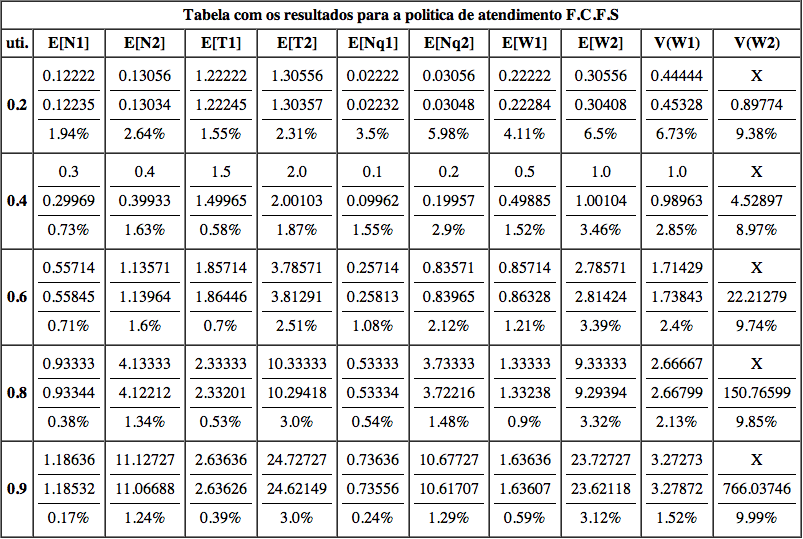
\includegraphics[width=1.0\textwidth]{tabelaFCFS.png}
   \caption{Tabela com os valores para a política de atendimento First Come First Served.}
\end{figure}

\pagebreak
\begin{figure}[htb!]
   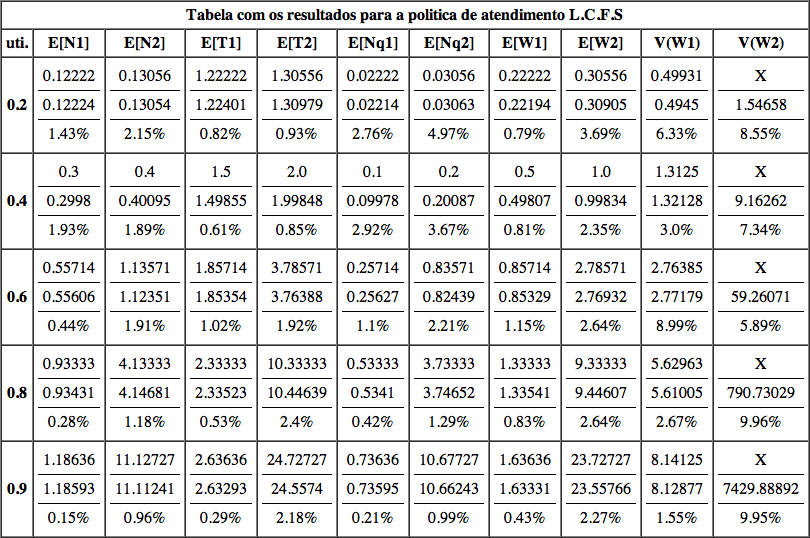
\includegraphics[width=1.0\textwidth]{tabelaLCFS.png}
   \caption{Tabela com os valores para a política de atendimento Last Come First Served.}
\end{figure}

\pagebreak

\section{Comentários}
\label{sec:coment}
aqui começa a seção comentários
